%%%%%%%%%%%%%%%%%%%%%%%%%%%%%%%%%%%%%%%%%
% Jacobs Landscape Poster
% LaTeX Template
% Version 1.1 (14/06/14)
%
% Created by:
% Computational Physics and Biophysics Group, Jacobs University
% https://teamwork.jacobs-university.de:8443/confluence/display/CoPandBiG/LaTeX+Poster
%
% Further modified by:
% Nathaniel Johnston (nathaniel@njohnston.ca)
%
% This template has been downloaded from:
% http://www.LaTeXTemplates.com
%
% License:
% CC BY-NC-SA 3.0 (http://creativecommons.org/licenses/by-nc-sa/3.0/)
%
%%%%%%%%%%%%%%%%%%%%%%%%%%%%%%%%%%%%%%%%%

%----------------------------------------------------------------------------------------
%	PACKAGES AND OTHER DOCUMENT CONFIGURATIONS
%----------------------------------------------------------------------------------------

\documentclass[final]{beamer}

\usepackage[scale=0.8]{beamerposter} % Use the beamerposter package for laying out the poster

\usetheme{confposter} % Use the confposter theme supplied with this template

\setbeamercolor{block title}{fg=ngreen,bg=white} % Colors of the block titles
\setbeamercolor{block body}{fg=black,bg=white} % Colors of the body of blocks
\setbeamercolor{block alerted title}{fg=white,bg=dblue!70} % Colors of the highlighted block titles
\setbeamercolor{block alerted body}{fg=black,bg=dblue!10} % Colors of the body of highlighted blocks
% Many more colors are available for use in beamerthemeconfposter.sty

%-----------------------------------------------------------
% Define the column widths and overall poster size
% To set effective sepwid, onecolwid and twocolwid values, first choose how many columns you want and how much separation you want between columns
% In this template, the separation width chosen is 0.024 of the paper width and a 4-column layout
% onecolwid should therefore be (1-(# of columns+1)*sepwid)/# of columns e.g. (1-(4+1)*0.024)/4 = 0.22
% Set twocolwid to be (2*onecolwid)+sepwid = 0.464
% Set threecolwid to be (3*onecolwid)+2*sepwid = 0.708

\newlength{\sepwid}
\newlength{\onecolwid}
\newlength{\twocolwid}
\newlength{\threecolwid}
\setlength{\paperwidth}{36in} % A0 width: 46.8in
\setlength{\paperheight}{24in} % A0 height: 33.1in
\setlength{\sepwid}{0.024\paperwidth} % Separation width (white space) between columns
\setlength{\onecolwid}{0.22\paperwidth} % Width of one column
\setlength{\twocolwid}{0.464\paperwidth} % Width of two columns
\setlength{\threecolwid}{0.708\paperwidth} % Width of three columns
\setlength{\topmargin}{-0.5in} % Reduce the top margin size
%-----------------------------------------------------------

\usepackage{graphicx}  % Required for including images

\usepackage{booktabs} % Top and bottom rules for tables

%----------------------------------------------------------------------------------------
%	TITLE SECTION
%----------------------------------------------------------------------------------------

\title{Exploring neural architectures for NER} % Poster title

\author{Vincent Billaut, Marc Thibault} % Author(s)

\institute{CS224n, Stanford University, 03/21/2018} % Institution(s)

%----------------------------------------------------------------------------------------

\begin{document}

\addtobeamertemplate{block end}{}{\vspace*{2ex}} % White space under blocks
\addtobeamertemplate{block alerted end}{}{\vspace*{2ex}} % White space under highlighted (alert) blocks

\setlength{\belowcaptionskip}{2ex} % White space under figures
\setlength\belowdisplayshortskip{2ex} % White space under equations

\begin{frame}[t] % The whole poster is enclosed in one beamer frame

\begin{columns}[t] % The whole poster consists of three major columns, the second of which is split into two columns twice - the [t] option aligns each column's content to the top

\begin{column}{\sepwid}\end{column} % Empty spacer column

\begin{column}{\onecolwid} % The first column

%----------------------------------------------------------------------------------------
%	OBJECTIVES
%----------------------------------------------------------------------------------------

% \begin{alertblock}{Objectives}

% Lorem ipsum dolor sit amet, consectetur, nunc tellus pulvinar tortor, commodo eleifend risus arcu sed odio:
% \begin{itemize}
% \item Mollis dignissim, magna augue tincidunt dolor, interdum vestibulum urna
% \item Sed aliquet luctus lectus, eget aliquet leo ullamcorper consequat. Vivamus eros sem, iaculis ut euismod non, sollicitudin vel orci.
% \item Nascetur ridiculus mus.
% \item Euismod non erat. Nam ultricies pellentesque nunc, ultrices volutpat nisl ultrices a.
% \end{itemize}

% \end{alertblock}

%----------------------------------------------------------------------------------------
%	INTRODUCTION
%----------------------------------------------------------------------------------------

\begin{block}{Motivation}
    \begin{itemize}
      \item NER with many classes is a complex task
      \item NER requires a thin understanding of context information
      \item We need to incorporate past and future dependencies
      \item A CRF implements a memory flow on labels
    \end{itemize}

\end{block}

%------------------------------------------------
\begin{block}{Dataset: CoNLL-2002}

Labelled new articles:

\vspace{5mm}

\begin{tabbing}
``\=The \=protest \=comes \=on \=the \=eve \=of \=the \=annual \=conference \\
\>\texttt{0} \>\texttt{0} \>\texttt{0} \>\texttt{0} \>\texttt{0} \>\texttt{0} \>\texttt{0} \>\texttt{0} \>\texttt{0} \>\texttt{0}
\end{tabbing}

\vspace{5mm}

\begin{tabbing}
of \=Britain\='s \=ruling \=Labor \=Party \= \ \=in \=the \=southern \\

\texttt{0} \>\texttt{B-geo} \>\texttt{0} \>\texttt{0} \>\texttt{B-org} \>\texttt{I-org} \> \>\texttt{0} \>\texttt{0} \>\texttt{0} 
\end{tabbing}

\vspace{5mm}

\begin{tabbing}
English \=seaside \=resort \=of \=Brighton. `` \\

\texttt{B-gpe} \>\texttt{0} \>\texttt{0} \>\texttt{0} \>\texttt{B-geo}
\end{tabbing}

\vspace{10mm}


\begin{itemize}
  \item $40,000$ train sentences,

  \item $10,000$ test sentences,

  \item $17$ label classes,

  \item Training takes $\sim$ 1h on multi-CPU.
\end{itemize}
\end{block}

%------------------------------------------------
\begin{block}{Base Models}

\begin{itemize}
  \item Words embedded with GloVe

  \item LSTM

  \item Bidirectional LSTM

  \item With(out) extra layer

  \item Cross-Entropy loss on labels

  \item Evaluation with $F_1$ score
\end{itemize}

\end{block}

\end{column} % End of the first column




\begin{column}{\sepwid}\end{column} % Empty spacer column

\begin{column}{\twocolwid} % Begin a column which is two columns wide (column 2)

\begin{columns}[t,totalwidth=\twocolwid] % Split up the two columns wide column

\begin{column}{\onecolwid}\vspace{-.6in} % The first column within column 2 (column 2.1)

%----------------------------------------------------------------------------------------
%	MATERIALS
%----------------------------------------------------------------------------------------

\begin{block}{Conditional Random Field}

  \begin{itemize}
  \item Encodes a Markov Chain: probability of transitioning from a label to another:

  \vspace{5mm}

  \[
  P[i, j] = Pr(y_{t+1} = y_j | y_{t} =y_i) \textit{ in training set}
  \]

  \vspace{5mm}

  $P$ stochastic matrix of size $(k,k)$.

  \vspace{10mm}

  \item Adds information to the prediction:

  \vspace{5mm}

  \begin{align*}
  z_0 &= argmax_j(\hat{y}_0[j])
  \\
  \text{and}&
  \\
  z_t &= argmax_j(\hat{y}_t[j] + \alpha.P[z_{t-1},  j]) \ \ \forall t \in [1, T]
  \end{align*}

  \vspace{5mm}

  $\alpha$ hyper-parameter which has to be fitted.

  \end{itemize}

\end{block}

%----------------------------------------------------------------------------------------

\end{column} % End of column 2.1

\begin{column}{\onecolwid}\vspace{-.6in} % The second column within column 2 (column 2.2)

%----------------------------------------------------------------------------------------
%	METHODS
%----------------------------------------------------------------------------------------

\begin{block}{Dropout rate selection}
\begin{center}
  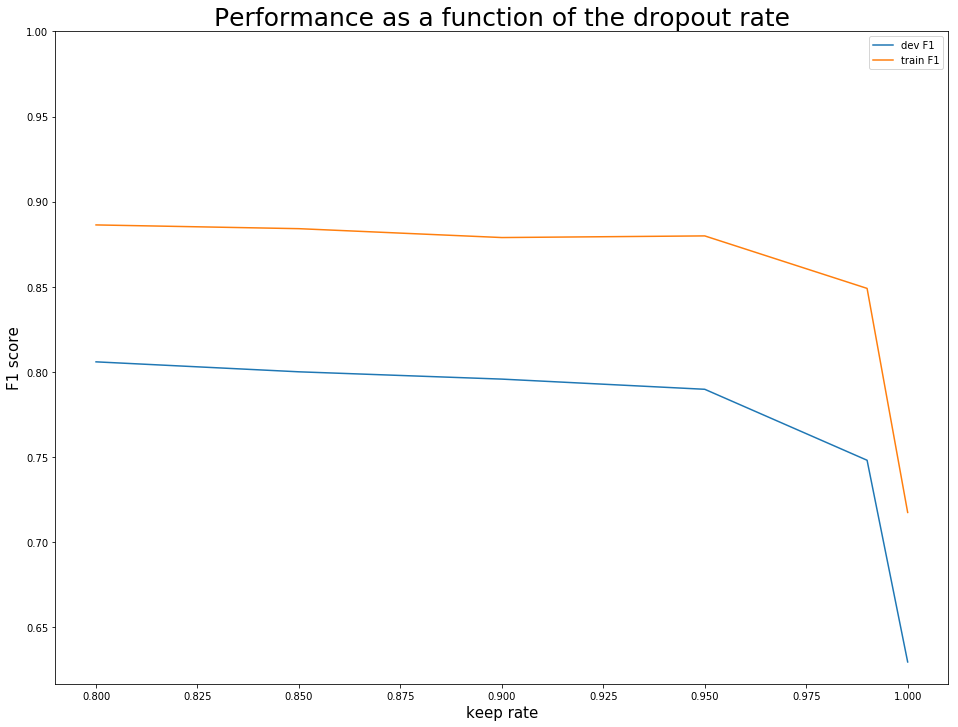
\includegraphics[scale=0.5]{figs/dr_graph.png}
\end{center}

We see that the dropout rate has a significant effect on the model's performance, and we therefore kept a value of \textbf{0.2} moving forward.

\end{block}

%----------------------------------------------------------------------------------------

\end{column} % End of column 2.2

\end{columns} % End of the split of column 2 - any content after this will now take up 2 columns width

% %----------------------------------------------------------------------------------------
% %	IMPORTANT RESULT
% %----------------------------------------------------------------------------------------

%\begin{alertblock}{Important Result}
%
%Lorem ipsum dolor \textbf{sit amet}, consectetur adipiscing elit. Sed commodo molestie porta. Sed ultrices scelerisque sapien ac commodo. Donec ut volutpat elit.
%
%\end{alertblock}

%----------------------------------------------------------------------------------------

\begin{columns}[t,totalwidth=\twocolwid] % Split up the two columns wide column again

\begin{column}{\onecolwid} % The first column within column 2 (column 2.1)

%----------------------------------------------------------------------------------------
%	MATHEMATICAL SECTION
%----------------------------------------------------------------------------------------

\begin{block}{Testing our models on five label dataset}

The scores reported in the papers we looked at are obtained by working on the same data as us, but with fewer labels (5 instead of 17). Although we chose to stick to the 17 labels version for our whole analysis, because we consider it to be more interesting (because more complex), we however tried to reach state-of-the-art performance on the "reduced" labels.

\begin{center}
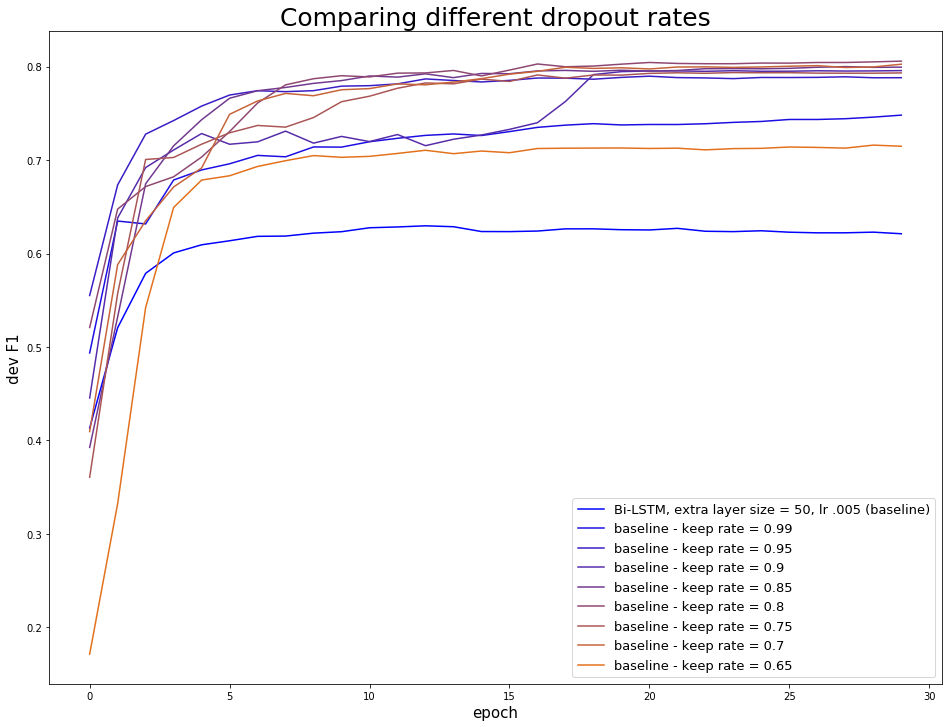
\includegraphics[scale=0.6]{figs/dr_devf1.png}
\end{center}

\end{block}

%----------------------------------------------------------------------------------------

\end{column} % End of column 2.1

\begin{column}{\onecolwid} % The second column within column 2 (column 2.2)

%----------------------------------------------------------------------------------------
%	RESULTS
%----------------------------------------------------------------------------------------

\begin{block}{L2 regularization study}

\begin{center}
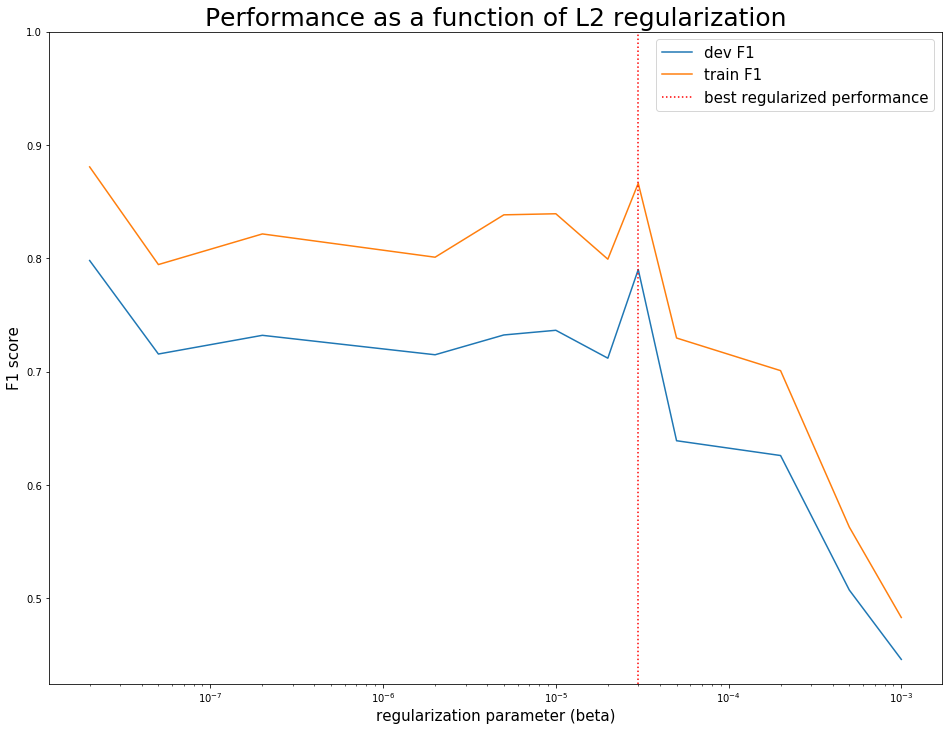
\includegraphics[scale=0.5]{figs/l2_graph.png}
\end{center}

Surprisingly, no regularized model significantly beats the baseline in terms of F1 score on the dev set. Still, we consider that introducing some regularization is safer for robustness, and therefore keep an L2 regularization parameter $\beta=3~10^{-5}$.

\end{block}

%----------------------------------------------------------------------------------------

\end{column} % End of column 2.2

\end{columns} % End of the split of column 2

\end{column} % End of the second column

\begin{column}{\sepwid}\end{column} % Empty spacer column

\begin{column}{\onecolwid} % The third column

%----------------------------------------------------------------------------------------
%	CONCLUSION
%----------------------------------------------------------------------------------------

\begin{block}{CRF performance}

  \begin{figure}
  \begin{center}
  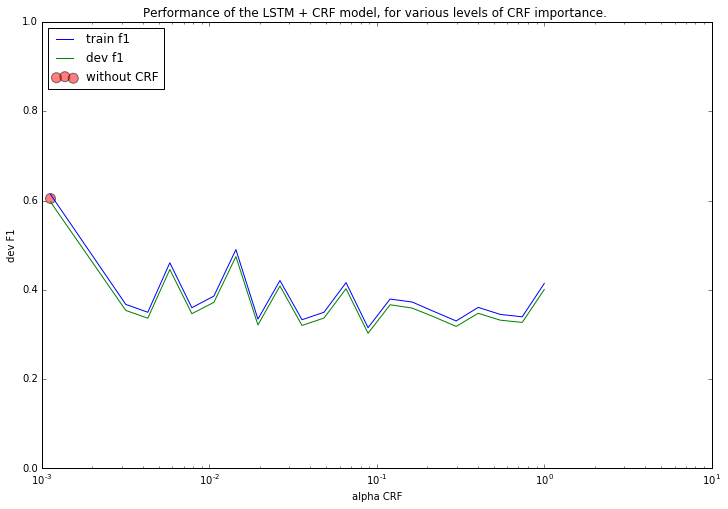
\includegraphics[width=600px]{figs/LSTM-CRF-vs-alpha.png}
  \caption{Train and Dev set performance of a LSTM model, incorporating a CRF on the prediction step, versus the importance $\alpha$ given to the CRF. No positive level of importance yields superior performance. The best decision is not to use the extra information from the CRF. }
  \label{lstm-crf-results}
  \end{center}
  \end{figure}

\end{block}

%----------------------------------------------------------------------------------------
%	ADDITIONAL INFORMATION
%----------------------------------------------------------------------------------------

% \begin{block}{Additional Information}

% Maecenas ultricies feugiat velit non mattis. Fusce tempus arcu id ligula varius dictum.
% \begin{itemize}
% \item Curabitur pellentesque dignissim
% \item Eu facilisis est tempus quis
% \item Duis porta consequat lorem
% \end{itemize}

% \end{block}

%----------------------------------------------------------------------------------------
%	REFERENCES
%----------------------------------------------------------------------------------------

\begin{block}{Results summary}

\begin{center}
   \begin{tabular}{||c | c||}
   \hline
   Model  & Dev $F_1$ \\
   \hline\hline
   Naive word-by-word & $0.691$ \\
   \hline
   LSTM & $0.597$ \\
   \hline
   LSTM + CRF & $0.475$ \\
   \hline
   LSTM + extra layer & $0.770$ \\
   \hline
   LSTM + extra layer + CRF & $0.751$ \\
   \hline
   Bi-LSTM & $0.796$ \\ [1ex]
   \hline
  \end{tabular}
\end{center}


\begin{center}
    
\includegraphics[scale=0.5]{figs/Stanford_logo}
\end{center}
\end{block}

%----------------------------------------------------------------------------------------
%	ACKNOWLEDGEMENTS
%----------------------------------------------------------------------------------------

% \setbeamercolor{block title}{fg=red,bg=white} % Change the block title color

% \begin{block}{Acknowledgements}

% \small{\rmfamily{Nam mollis tristique neque eu luctus. Suspendisse rutrum congue nisi sed convallis. Aenean id neque dolor. Pellentesque habitant morbi tristique senectus et netus et malesuada fames ac turpis egestas.}} \\

% \end{block}

%----------------------------------------------------------------------------------------
%	CONTACT INFORMATION
%----------------------------------------------------------------------------------------

% \setbeamercolor{block alerted title}{fg=black,bg=norange} % Change the alert block title colors
% \setbeamercolor{block alerted body}{fg=black,bg=white} % Change the alert block body colors

% \begin{alertblock}{Contact Information}

% \begin{itemize}
% \item Web: \href{http://www.university.edu/smithlab}{http://www.university.edu/smithlab}
% \item Email: \href{mailto:john@smith.com}{john@smith.com}
% \item Phone: +1 (000) 111 1111
% \end{itemize}

% \end{alertblock}

% \begin{center}
% \begin{tabular}{ccc}
% \includegraphics[width=0.4\linewidth]{logo.png} & \hfill & \includegraphics[width=0.4\linewidth]{logo.png}
% \end{tabular}
% \end{center}

%----------------------------------------------------------------------------------------

\end{column} % End of the third column

\end{columns} % End of all the columns in the poster

\end{frame} % End of the enclosing frame

\end{document}
